\documentclass%[handout]%
{beamer}
%\usetheme{Execushares}
\usetheme{AnnArbor}
\usecolortheme{beaver}
%\setbeamercolor{title}{parent=structure,bg=green!50!black,fg=white}
%\usecolortheme{dolphin}
\setbeamertemplate{navigation symbols}{}%remove navigation symbols

\usepackage{amsmath}
\usepackage{amssymb}
\usepackage{amsthm}
%\usepackage[utf8]{inputenc}
\usepackage[czech]{babel}
\usepackage{tikz-cd}
\usepackage[mathscr]{euscript}
\usepackage[IL2]{fontenc}
\usepackage{mathtools}
\usepackage[normalem]{ulem}

\usetikzlibrary{calc,shapes.callouts,shapes.arrows}

%\usepackage{beamerarticle}

%\usepackage{bbm}

\def\rllap#1{\hbox to0pt{\hss#1\hss}}

%\newcommand{\bubblethis}[2]{
        %\tikz[remember picture,baseline]{\node[anchor=base,inner sep=0,outer sep=0]%
        %(#1) {\underline{#1}};\node[overlay,cloud callout,callout relative pointer={(-0.2cm,+0.7cm)},%
        %aspect=2.5,fill=yellow!90] at ($(#1.north)+(-0.5cm,1.6cm)$) {#2};}%
    %}%
		%
%\newcommand{\speechthis}[2]{
        %\tikz[remember picture,baseline]{\node[anchor=base,inner sep=0,outer sep=0]%
        %(pom) {#1};\node[overlay,ellipse callout,fill=blue!50] 
        %at ($(pom.north)+(1cm,+0.8cm)$) {#2};}%
    %}%
		
\newcommand{\R}{\mathbb R}

%\title{Limity funkcí}
\author{Alexander Slávik} %  and J. Trlifaj
\title{Asymptoty, spojitost na intervalu}
\institute{Gymnázium Voděradská}
\date{18. 11. 2020}

\begin{document}





\section{Asymptoty}

\begin{frame}
	\frametitle{Asymptoty}
	\pause
	\uv{Přímky, k nimž se graf funkce blíží.}\pause
	\[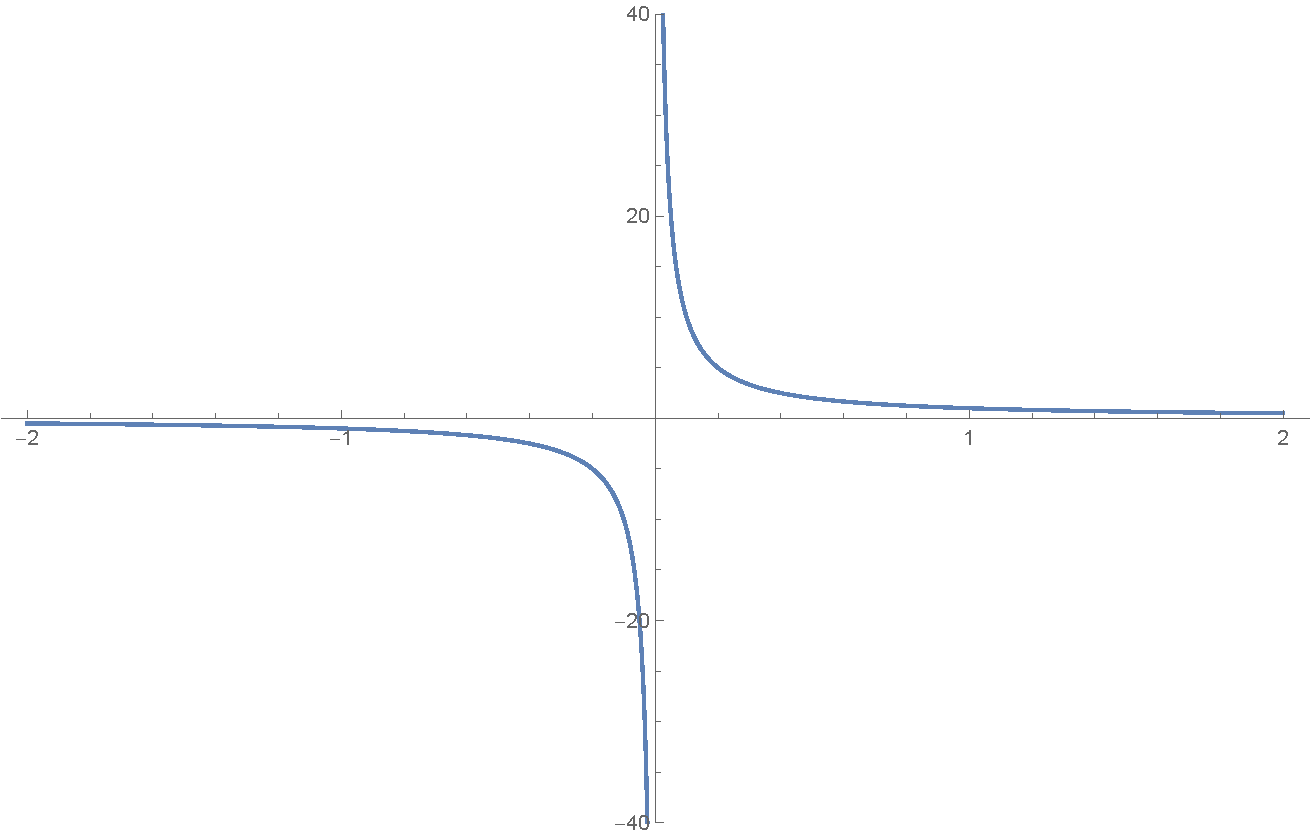
\includegraphics[height=.6\vsize]{grafy/invzero.pdf}\]
	\pause
	Funkce $y = \frac1x$ má asymptoty $x = 0$ (svislá) a $y = 0$ (vodorovná).
\end{frame}



\begin{frame}
	\frametitle{Dva druhy asymptot}
	\pause
	\[ \text{asymptoty} \begin{cases}\pause
	\text{bez směrnice}\\ \pause
	\text{se směrnicí}
	\end{cases}\]
\end{frame}
	
\begin{frame}
	\frametitle{Asypmtota bez směrnice}		
	\begin{block}{Definice}
	Přímka $x = a$ se nazývá \emph{asymptotou bez směrnice grafu funkce $f$}, existuje-li aspoň jedna z limit
	\[ \lim_{x \to a_+}f(x), \qquad \lim_{x \to a_-}f(x) \]
	a je nevlastní (tj. rovna $\pm \infty$).
	\end{block}\pause
	\vskip-.25cm
	\[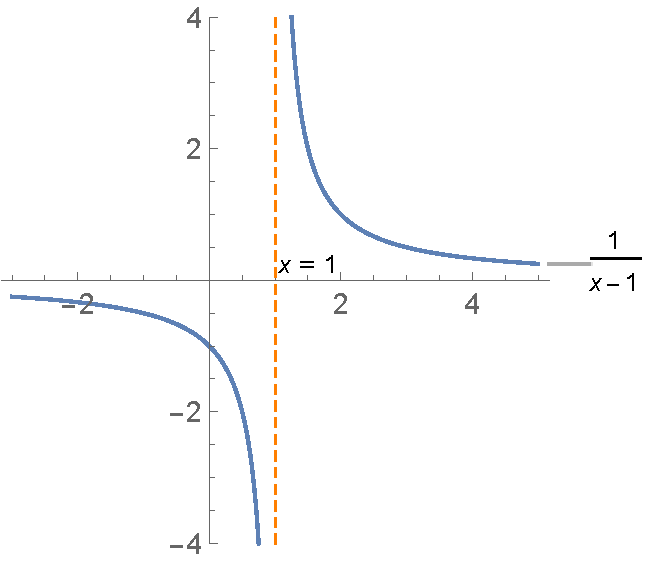
\includegraphics[height=.4\vsize]{grafy_asy/vert_asy.pdf} \qquad\pause 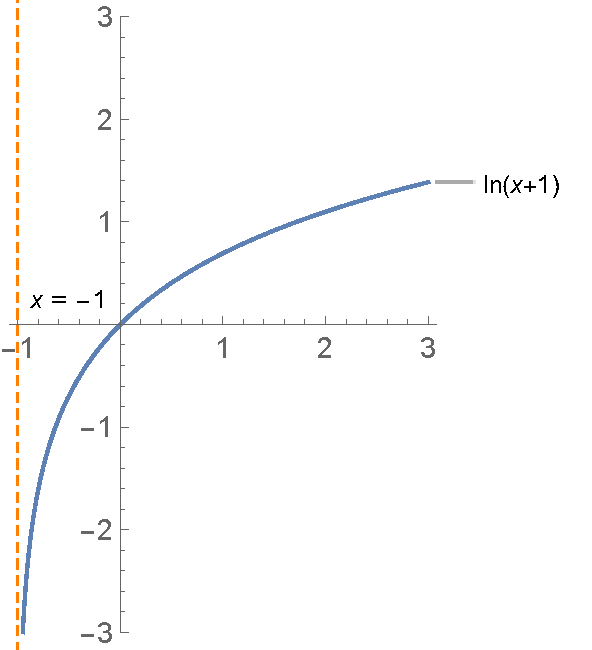
\includegraphics[height=.4\vsize]{grafy_asy/vert_asy_log.pdf}\]
\end{frame}


\begin{frame}
	\frametitle{Asypmtota se směrnicí}		
	\begin{block}{Definice}
	Přímka $y = ax + b$ (kde $a, b \in \R$) se nazývá \emph{asymptotou se směrnicí grafu funkce $f$}, platí-li
	\[ \lim_{x \to \infty}(f(x) - (ax+b)) = 0 \quad \text{nebo}\quad \lim_{x \to -\infty}(f(x) - (ax+b)) = 0. \]
	\end{block}\pause
	\vskip-5mm
	\[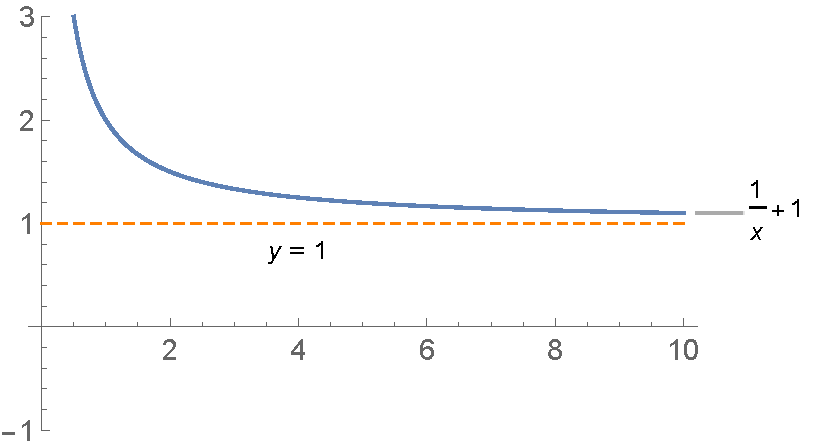
\includegraphics[height=.4\vsize]{grafy_asy/hor_asy_1.pdf} \qquad\pause 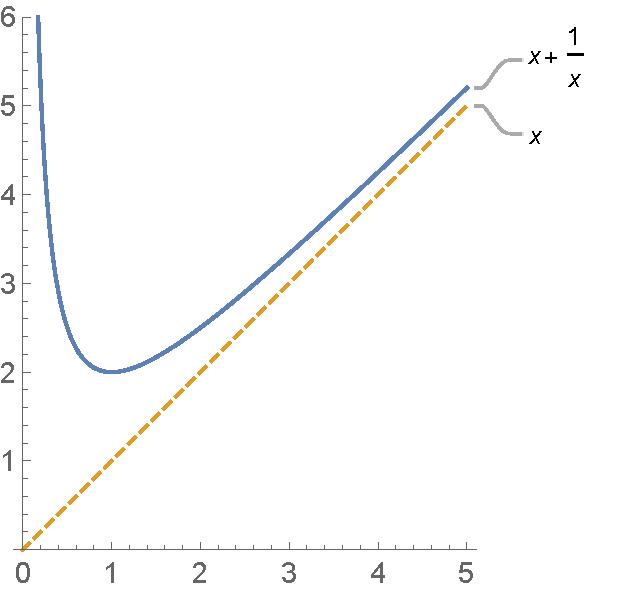
\includegraphics[height=.5\vsize]{grafy_asy/hor_asy_2.pdf}\]
\end{frame}

\begin{frame}
	\frametitle{Výpočet asypmtoty se směrnicí}
	\pause
	\begin{enumerate}
		\item Spočteme $a = \lim\limits_{x \to \infty} \frac{f(x)}{x}$. \pause
		Pokud tato limita existuje a je vlastní, pokračujeme.\pause
		\item Spočteme $b = \lim\limits_{x \to \infty} f(x) - ax$. \pause Pokud tato limita existuje a je vlastní, je $y = ax + b$ asymptotou (se směrnicí).
	\end{enumerate}
	\pause
	Pokud nám v jednom z kroků nevyšla vlastní limita, asymptota se směrnicí (v $\infty$) neexistuje. \pause Stejně se to provede pro $-\infty$.
\end{frame}


\begin{frame}
	\frametitle{Asymptoty se směrnicí mohou být různé!}
	\[ f\colon y = \frac{x}{2^x+1} + x \]
	\pause
	\[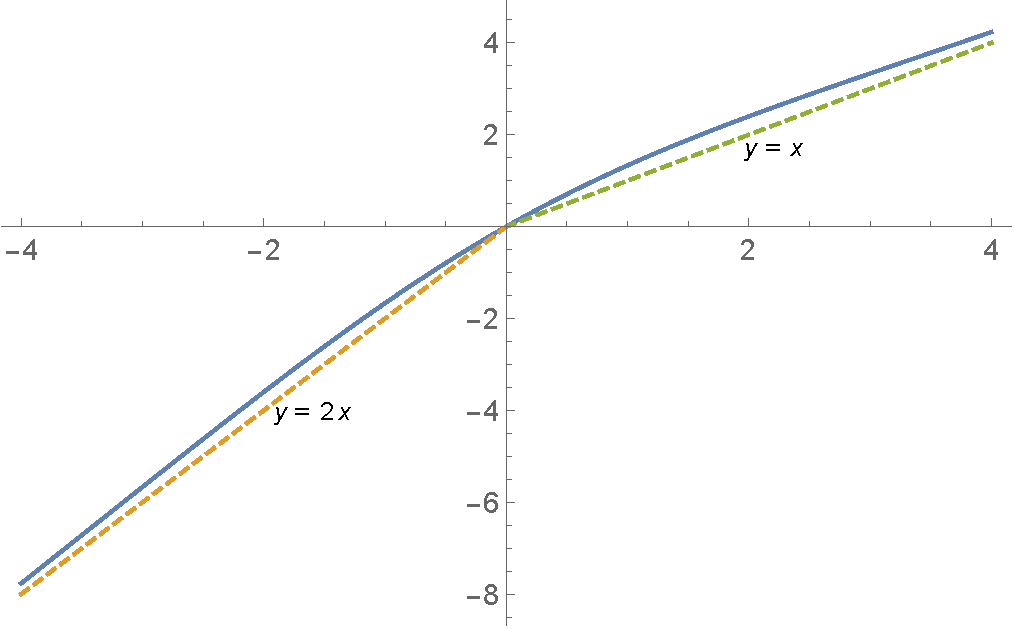
\includegraphics[height=.6\vsize]{grafy_asy/diff_asy.pdf}\]
\end{frame}


\section{Funkce spojité na intervalu}

\begin{frame}
	\frametitle{Spojitost podruhé}
	Připomeňme, že funkce $f$ je \emph{spojitá v bodě $a \in D_f$}, pokud platí $\lim\limits_{x \to a}f(x) = f(a)$.
	
	\pause\medskip
	Přidáme ještě:
	\begin{itemize}
		\item zprava spojitá v $a$: $\lim\limits_{x \to a_+}f(x) = f(a)$,
		\item zleva spojitá v $a$: $\lim\limits_{x \to a_-}f(x) = f(a)$.
	\end{itemize}
	
	%\bigskip
	\pause
	\begin{block}{Definice}
	Je-li $I$ interval, pak řekneme, že $f$ \emph{je spojitá na $I$}, pokud je spojitá v~každém vnitřním bodě $I$, případně jednostranně spojitá v krajních bodech, pokud patří do $I$.
	\end{block}
	
	%\bigskip
	\pause
	Funkce spojitá na intervalu $I$ $\approx$ \textcolor{pink}{\emph{\uv{jde na $I$ nakreslit jedním tahem}}}.
\end{frame}


\begin{frame}
	\frametitle{Spojitá funkce na uzavřeném intervalu nabývá extrémů}
	
	\pause
	
	\begin{block}{Věta}
	Nechť $a$, $b$ jsou reálná čísla splňující $a < b$ a funkce $f$ je spojitá na intervalu $\langle a; b\rangle$. \pause Pak existují $m, M \in \langle a; b\rangle$ taková, že pro všechna $x \in \langle a; b\rangle$ platí
	\[ f(m) \leq f(x) \leq f(M). \]
	\end{block}
	
	\pause
	Speciálně je spojitá funkce na uzavřeném intervalu omezená.
	
	\pause \bigskip
	Je nutné, aby byl interval \alert{uzavřený}!
\end{frame}


\begin{frame}
	\frametitle{Spojitá funkce nabývá mezihodnot}
	
	\pause
	
	\begin{block}{Věta}
	Nechť $a$, $b$ jsou reálná čísla splňující $a < b$ a funkce $f$ je spojitá na intervalu $\langle a; b\rangle$. Pak pro každé $y$ mezi $f(a)$ a $f(b)$ existuje $c \in \langle a; b \rangle$ splňující $f(c) = y$.
	\end{block}
	
	\pause
	
	\begin{exampleblock}{Důsledek}
	Je-li $f$ spojitá na $\langle a; b\rangle$ a platí buď $f(a) \leq 0$ a $f(b) \geq 0$, nebo $f(a) \geq 0$ a $f(b) \leq 0$, tak existuje $c \in \langle a; b\rangle$ splňující $f(c) = 0$.
	\end{exampleblock}
\end{frame}


%\end{document}

\begin{frame}
	\frametitle{Půlení intervalů}
	\dots aneb \uv{Jak vyřešit libovolnou rovnici.}
	\pause
	
	
	\bigskip
	\begin{enumerate}
		\item Rovnici převedeme do tvaru $f(x) = 0$. \pause (Předpokládáme, že $f$ je spojitá na dostatečně velkém intervalu.)\pause
		\item Odhadneme body $a, b \in \R$ takové, že hodnoty $f(a)$ a $f(b)$ mají opačné znaménko.\pause
		\item Podíváme se do bodu $c = \frac{a+b}{2}$. \pause Mají-li $f(c)$ a $f(a)$ stejné znaménko, pak nahradíme $a$ za $c$ a pokračujeme předchozím bodem. \pause Mají-li $f(c)$ a $f(a)$ různé znaménko, pak nahradíme $b$ za $c$ a pokračujeme předchozím bodem.\pause
		\item Opakujeme body 2 a 3, dokud nemáme tak přesný výsledek, jak bychom chtěli.
	\end{enumerate}
	
	
	
	
\end{frame}



\end{document}
